%!TEX root = lec06_transactions.tex

%%%%%%%%%%%%%%% ---- 

%
% ---------------------------------
%
\begin{frame}{Locking? Timestamping?}

There is no \textbf{single} model that is best for all applications. 

The choice depends on the \textbf{mix of queries and updates} in the workload.

\vskip1em

\begin{center}
\framebox{\parbox{0.825\textwidth}{The only low hanging fruit here: if the workload is 100\% of queries, there is no need for concurrency control!}}
\end{center}

\vskip1em

Many systems use a \textbf{combination} of locking and timestamping:
\begin{itemize}[-,noitemsep]
 \item 2PL with shared locks to execute updates
 \item timestamping with multiple versions for queries
\end{itemize}
\end{frame}

%
% ---------------------------------
%
\begin{frame}{Overhead of ensuring Isolation}

\begin{center}
\framebox{$E$: number of database elements; $T$: number of transactions}
\end{center}

Space cost of implementing isolation. 

\textbf{Locking}: $O(E \cdot T)$\\
 - lock table grows linearly with the number of locked elements

\textbf{Timestamping}: $O(E) + O(T)$\\
 - read/write times for each element and timestamps for each transaction

\textbf{Timestamping + versioning}: $O(E\cdot T)$\\
 - every transaction may create a new version of every element

\end{frame}

%
% ---------------------------------
%
\begin{frame}

In all concurrency control models, some steps must be done \textbf{atomically} by the scheduler:
\begin{itemize}[-,noitemsep]
\item updating the lock table
\item updating the timestamp table
\item creating/deleting versions
\end{itemize}

These operations require \textbf{synchronization} and cannot be done in parallel to avoid race conditions leading to inconsistency, which can limit the system throughput.
\end{frame}

%
% ---------------------------------
%
\begin{frame}{Isolation Levels in SQL}
SQL allows \textbf{\alert{the programmer} to chose the level of isolation} necessary for \underline{each transaction} in the application.

In SQL:1999 these isolation levels are possible:
\begin{itemize}[-,noitemsep,topsep=-0.5em]
\item \lstinline[style=SQL]{READ UNCOMMITTED}: the transaction is allowed to perform dirty reads.
\item \lstinline[style=SQL]{READ COMMITTED}: the transaction can only read elements that have been committed.
\item \lstinline[style=SQL]{REPEATABLE READ}: database elements read by the transaction cannot change after it starts.
\item \lstinline[style=SQL]{SERIALIZABLE}: the transaction runs in total isolation from other transactions.
\end{itemize}
\end{frame}

%
% ---------------------------------
%
\begin{frame}{SQL isolation levels and the problems they prevent}

\begin{center}
% \large
\begin{tabular}{p{2cm}cp{3cm}c}
\textbf{Level} &  \textbf{dirty reads} & \textbf{non-repeatable reads} & { \textbf{phantoms}} \\
\lstinline[style=SQL]{READ} \lstinline[style=SQL]{UNCOMMITTED} & 
\cellcolor{red!15}  \raisebox{-0.75em}{allows} & 
\cellcolor{red!15}  \centering \raisebox{-0.75em}{allows} &
\cellcolor{red!15}  \raisebox{-0.75em}{allows} \\
\hline
\lstinline[style=SQL]{READ} \lstinline[style=SQL]{COMMITTED} & 
\cellcolor{green!15}  \raisebox{-0.75em}{prevents} & 
\cellcolor{red!15}  \centering \raisebox{-0.75em}{allows} &
\cellcolor{red!15}  \raisebox{-0.75em}{allows} \\
\hline
\lstinline[style=SQL]{REPEATABLE} \lstinline[style=SQL]{READ} & 
\cellcolor{green!15}  \raisebox{-0.75em}{prevents} & 
\cellcolor{green!15}  \centering \raisebox{-0.75em}{prevents} &
\cellcolor{red!15}  \raisebox{-0.75em}{allows} \\
\hline
\raisebox{-0.75em}{\lstinline[style=SQL]{SERIALIZABLE}} & 
\cellcolor{green!15}  \raisebox{-0.75em}{prevents} & 
\cellcolor{green!15}  \centering \raisebox{-0.75em}{prevents} &
\cellcolor{green!15}  \raisebox{-0.75em}{prevents} \\[1.5em]
\end{tabular}
\end{center}

\end{frame}

\begin{frame}{Preventing Dirty Reads}

As we saw, both locking and timestamp-based concurrency control prevent dirty reads.

\vskip2em

An even simpler (and faster) solution would be to use just the \textbf{commit bits} \C{X} of the timetamp concurrency control approach. 

\end{frame}

%
% ---------------------------------
%
\begin{frame}

\vskip1em

\begin{columns}[onlytextwidth]
\begin{column}{0.6\textwidth}
Aside: are \textbf{dirty reads} a real problem?
\end{column}
\begin{column}{0.4\textwidth}
\begin{center}

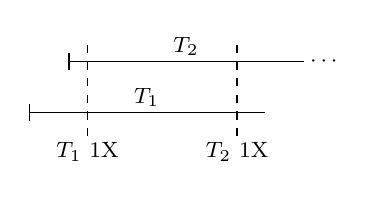
\begin{tikzpicture}[semithick,every node/.append style={font=\footnotesize}]
\begin{scope}[>=latex]
\draw [|-] (0.5,1) -- (3.5,1) node [midway,yshift=-5pt,label=above:{$T_1$}] {};
\draw [|-] (1,1.65) -- (4,1.65) node [midway,yshift=-5pt,label=above:{$T_2$}] {};
\node at (3.75,1) {\ABORT};
\node at (4.25,1.65) {$\cdots$};
\end{scope}

\draw[dashed] (1.25,0.7) -- (1.25,1.9); % t1 writes (X)
\node (1) at (1.25,0.5) {$T_1$ \W{1}{X}};

\draw[dashed] (3.15,0.7) -- (3.15,1.9); % t1 reads (X)
\node (1) at (3.15,0.5) {$T_2$ \R{1}{X}};

\end{tikzpicture}
\end{center}
\end{column}
\end{columns}


\alert{\textbf{DEFINITELY YES}} for applications like \alert{banking}:
\begin{itemize}[-,noitemsep,topsep=-5pt]
 \item $T_1$ is a deposit; $T_2$ is a withdrawal from the same account.
 \item The dirty read may authorize the ATM to dispense money that the customer does not have
\end{itemize}

\vskip1em

\blue{\textbf{MAYBE?}} for \alert{OLAP workloads (``analytics'', business intelligence)}:
\begin{itemize}[-,noitemsep,topsep=-5pt]
 \item $T_1$ is a sale of \emph{items}; $T_2$ generates a monthly sales report
 \item The dirty read will overestimate the monthly sales of those items, which might not be a problem
\end{itemize}
\end{frame}

%
% ---------------------------------
%


\begin{frame}{Non-Repeatable Read}

A \textbf{Non-Repeatable Read} (NRR) happens when \underline{two reads} of the \alert{same database} element by the \alert{same transaction} return \underline{different values}.

\vskip1em

\begin{center}
\scalebox{0.9}{\usebox{\longRunningNRRexample}}
\end{center}

\vskip1em

As we saw, all methods can detect and prevent NRRs.

Although snapshot isolation (MVCC) prevents NRRs at the expense of potential inconsistencies.
\end{frame}

%
% ---------------------------------
%


\begin{frame}{Phantom tuples}

Happen when a transaction $T_1$ reads from a relation that another transaction $T_2$ is inserting new tuples to.

\vskip1em
\begin{block}{Typical example}
$T_1$  computes an aggregate over a column of relation $R$ while $T_2$, at the same time, \alert{inserts new tuples} in $R$.
\end{block}

\vskip1em
\begin{center}
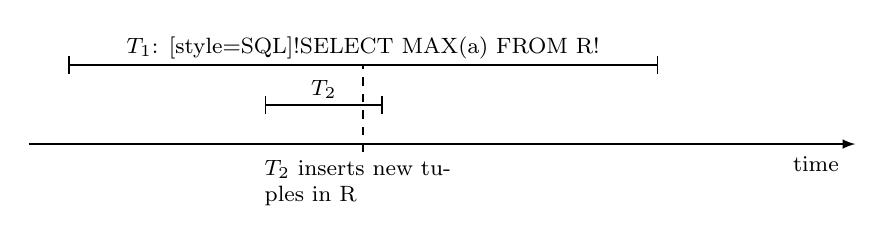
\begin{tikzpicture}[semithick,every node/.append style={font=\footnotesize}]
\begin{scope}[>=latex]
\draw [->] (0,1.5) -- (10.5,1.5); \node (caption) at (10,1.25) {time};
\draw [|-|] (0.5,2.5) -- (8,2.5) node [midway,yshift=-5pt,label=above:{$T_1$: \lstinline[style=SQL]!SELECT MAX(a) FROM R! }] {};
\draw [|-|] (3,2) -- (4.5,2) node [midway,yshift=-5pt,label=above:{$T_2$}] {};
\end{scope}

\draw[dashed] (4.25,1.4) -- (4.25,2.5); 
\node [text width=2.5cm] at (4.25,1.0) {$T_2$ inserts new tuples in R};
\end{tikzpicture}
\end{center}

\end{frame}

\begin{frame}

Locking and timestamp based concurrency control work at the level of database elements (e.g., tuples or attributes of tuples). However...
\begin{itemize}[-,noitemsep,topsep=-5pt]
\item $T_1$ cannot lock the tuples inserted by $T_2$ because it does not even know they exist!
\item There are no read/write violations involving them either.
\end{itemize}

\pause

\vskip1em

\textbf{Solution}: $T_2$  must lock the \underline{entire relation} before it can go through with the insertion.

\vskip1em

\vskip1em
\begin{center}
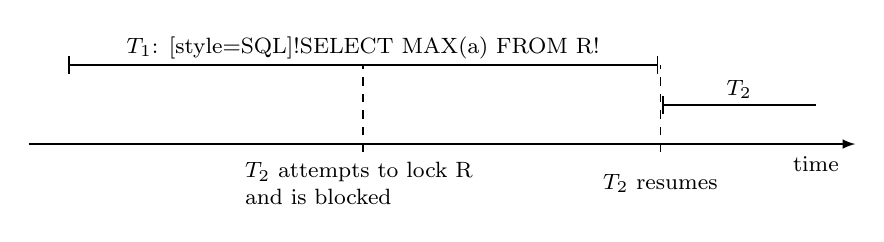
\begin{tikzpicture}[semithick,every node/.append style={font=\footnotesize}]
\begin{scope}[>=latex]
\draw [->] (0,1.5) -- (10.5,1.5); \node (caption) at (10,1.25) {time};
\draw [|-|] (0.5,2.5) -- (8,2.5) node [midway,yshift=-5pt,label=above:{$T_1$: \lstinline[style=SQL]!SELECT MAX(a) FROM R! }] {};
\draw [|-] (8.05,2) -- (10,2) node [midway,yshift=-5pt,label=above:{$T_2$}] {};
\end{scope}

\draw[dashed] (4.25,1.4) -- (4.25,2.5); % t2 writes (X)
\node [text width=3cm] at (4.25,1.0) {$T_2$ \blue{attempts to lock R} and is \alert{blocked} };

\draw[dashed] (8.025,1.4) -- (8.025,2.5); % t2 writes (X)
\node [] at (8.025,1.0) {$T_2$ resumes};
\end{tikzpicture}
\end{center}

\end{frame}

